% Define document class
\documentclass[twocolumn]{aastex631}
\DeclareRobustCommand{\Eqref}[1]{Eq.~\ref{#1}}
\DeclareRobustCommand{\Figref}[1]{Fig.~\ref{#1}}
\DeclareRobustCommand{\Tabref}[1]{Tab.~\ref{#1}}
\DeclareRobustCommand{\Secref}[1]{Sec.~\ref{#1}}
% \usepackage{cuted}
% \usepackage{flushend}
\usepackage{amsmath}
% \graphicspath{{./figures/}}

\begin{document}

% Title
\title{Simulated Velocity Dispersion of Bar Stars in the Milky Way–M31 Merger}

\author[0009-0008-2061-4946]{C.~A.~Burt}
\affiliation{University of Arizona, Department of Astronomy \& Steward Observatory, 933 N.~Cherry Ave., Tucson, AZ 85721, USA}

\correspondingauthor{C.~A.~Burt}
\email{caburt@arizona.edu}

% \begin{abstract}
% \end{abstract}

\section{Introduction}

\textbf{Major mergers} in cosmology refer to the collision and
subsequent consolidation of two spiral galaxies of similar size
\citep[e.g.,][]{mutch:11}. They represent one of the most dramatic
processes that can alter the characteristics of a galaxy. The
\textbf{dynamical friction} generated from individual gravitational
force interactions between stars in each galaxy are great enough to
destroy the elongated collection of stars near the center of each
galaxy that fuels the galactic nucleus called the \textbf{stellar bar}
\citep[e.g.,][]{knapen:02}. Concurrently, major mergers destroy the
dense spiral arms composed of young stars that define a \textbf{spiral
  galaxy} and convert it into an \textbf{elliptical galaxy}. which are
identified by their ellipsoidal structure and older stellar population
\citep{hubble:36}. Major mergers encapsulate a broader area of
galactic structure and dynamics and by analyzing the evolution of
stellar bars, we gain insight into the mechanisms that drive the
overall transformation of galaxies \citep[e.g.,][]{vandermarel:01}.

This topic is central to our understanding of the processes by which
galaxies change over time, or \textbf{galactic evolution}. The
disruption or alteration of the bar structure plays a critical role in
the transformation of galactic geometry \citep{wu:18}. After all, the
definition of a galaxy as defined by \citet{willman:12} states ``A
galaxy is a \textbf{gravitationally bound} set of stars whose
properties cannot be explained by a combination of baryons (gas, dust
and stars) and Newton’s laws of gravity'', where ``gravitationally
bound'' describes a system where the gravitational potential energy is
stronger than the potential energy. Bar dynamics, while concerning a
small fraction of the galactic population, exemplifies a region that
demands scrutiny as the definition from \citet{willman:12}
suggests. Furthermore, the presence and nature of bars significantly
affects star formation and the secular evolution of galaxies
\citep{schoenrich:17}. Understanding how mergers affect these
structures helps elucidate the processes that cause barred spiral
galaxies to transition into elliptical galaxies, ultimately shaping
the observable characteristics of galaxies in the universe.

Current research indicates that major galactic mergers prompt
significant changes in spiral galaxies, frequently leading to an
evolution towards an elliptical shape
\citep[e.g.,][]{mutch:11}. Although simulations have successfully
replicated some aspects of this transformation, the details of the
intermediate stages remain poorly understood \citep{berentzen:03}. The
prevailing view is that the bar structure, characteristic of many
spiral galaxies, is significantly disrupted during mergers
\citep[e.g.,][]{mihos:96,mutch:11}. The dynamics of stars within the
bar are disturbed, leading to a chaotic dispersal throughout the
merged galaxy. As shown in \Figref{fig:elmegreen}. Despite a
qualitative understanding of the overall process, there exist gaps in
our knowledge of the precise mechanisms at work.

\begin{figure}[htbp]
    \centering
    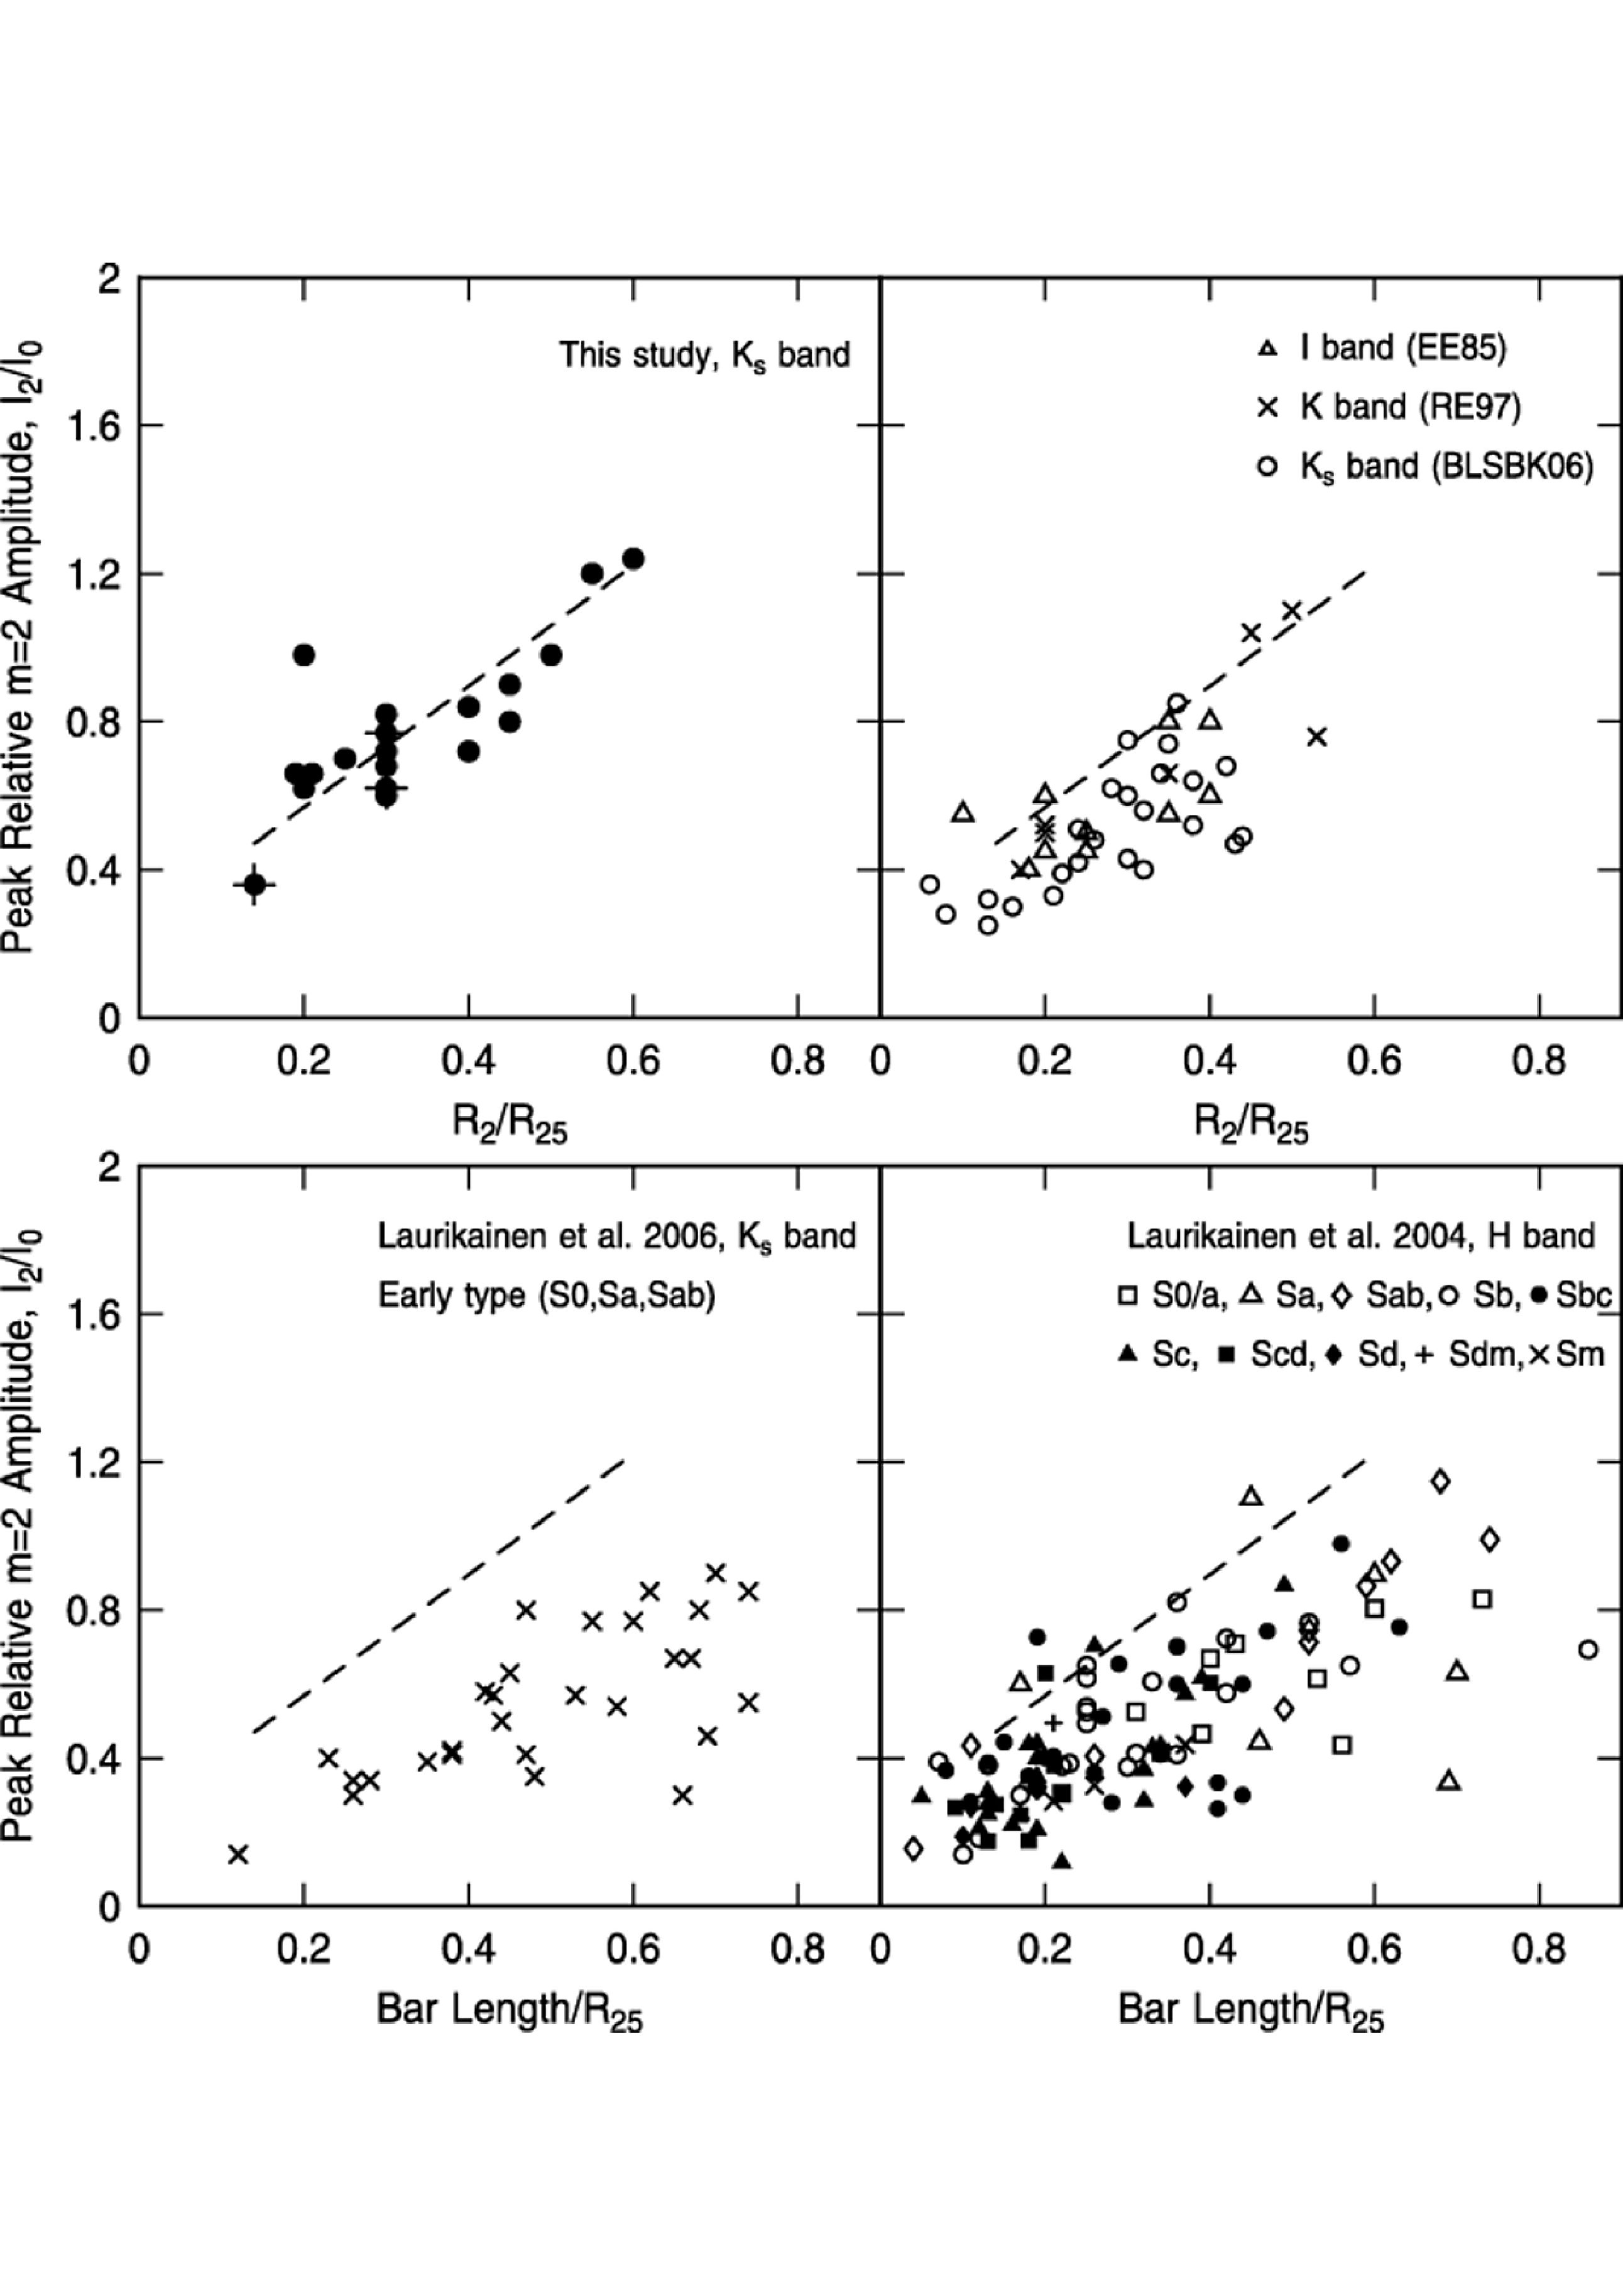
\includegraphics[width=\columnwidth]{elmegreen07}
    \caption{Figure 2 from \citet{elmegreen:07}. Peak relative
      amplitude of the Fourier component vs. the normalized radius at
      the peak. The different windows show galactic surveys delineated
      by emission detected \citep[see][]{elmegreen:07}. For all
      surveys, the bars that have higher peak relative amplitudes of
      the Fourier component are longer compared to their galaxy size.}
    \label{fig:elmegreen}
\end{figure}


Despite progress in simulating and observing galactic mergers, several
open questions persist. The exact physical measurements and
properties of bar structures in spiral galaxies are the subject of an
ongoing debate, which greatly influences the evolution of galactic
centers during a merger \citep{rathore:25}. Furthermore, it is partially unclear
how individual perturbations during a merger contribute to the overall
disruption of the bar, and how we can predict the detailed dynamics of
these events \citep{berentzen:03}. Addressing these uncertainties is vital for
developing a more comprehensive model of galaxy evolution post-merger,
ultimately enhancing our understanding of the lifecycle of galaxies.

\begin{figure}[htbp]
  \centering
  \includegraphics[width=\columnwidth]{dehnen23.jpeg}
  \caption{Figure 7 from \citet{dehnen:23}. The visual demonstrates
    one method used to determine the bar size and shape. This figure
    is generated from simulation snapshots, which mirrors the method I
    discuss later in the proposal.}
  \label{fig:dehnen}
\end{figure}

\section{This Project}

Here, we study the influence the major merger predicted between the
Milky Way and Andromeda (M31) galaxies as simulated in
\citet{vandermarel:12} has on the strength of the peak of the Fourier
amplitude in each constituent galaxy.

We use a modified classification for the stellar bar from
\citet{dehnen:23} to determine how force interactions between stars
contribute to the overall disruption of the bar during a major merger.

The destruction of a bar indicates the evolution from a barred spiral
galaxy to an elliptical galaxy. With respect to this, the overall
structure of a galaxy dependent on the strength of a bar if present
and understanding the evolution of the bar is tantamount to
understanding galactic evolution in terms of galactic shape, star
formation, and the ultimate fate of the Local Group.

\section{Methodology}
This manuscript uses data from \citet{vandermarel:12}. This is an
optimized N-body simulation containing stars in the disk and bulge of
MW, M31, and M33. An N-body simulation is a simulation in which each
timestep involves a gravitational force calculation between each
particle and all other particles, finding the net acceleration and
applying that to an orbit integration method. \citet{vandermarel:12}
optimizes this method by grouping together weak force interactions
that influence a particle in the same direction and neglecting very
weak force interactions. This simulation models the dynamics of the
Local Group as it experiences a major merger.

To perform any analysis on the barred region of a spiral galaxy, one
must first define the bar. As previously discussed, this remains an
active area of research \citep{berentzen:03}. For this project, I
employ the method depicted in \Figref{fig:dehnen} from
\citet{dehnen:23} due to our analogous methodologies. This approach
requires an input parameter $\theta$ that I obtain from the location
of high-density regions in \Figref{fig:spiral}. For this paper, I use
the high-resolution positional disk and bulge star data from
\citet{vandermarel:12} to employ the method from
\citet{dehnen:23}. After identifying the stars located in their host
galaxy's bar, I write a function that identifies close encounters
between the Milky Way and M33 and generates a list of snapshots with
an interval of 16 at ``quiet'' intervals, an interval of 1 surrounding
close encounters and interval sizes of 2, 4, and 8 to provide smooth
transitions. At each snapshot, I calculate the bar strength.

\begin{figure}[htbp]
  \centering
  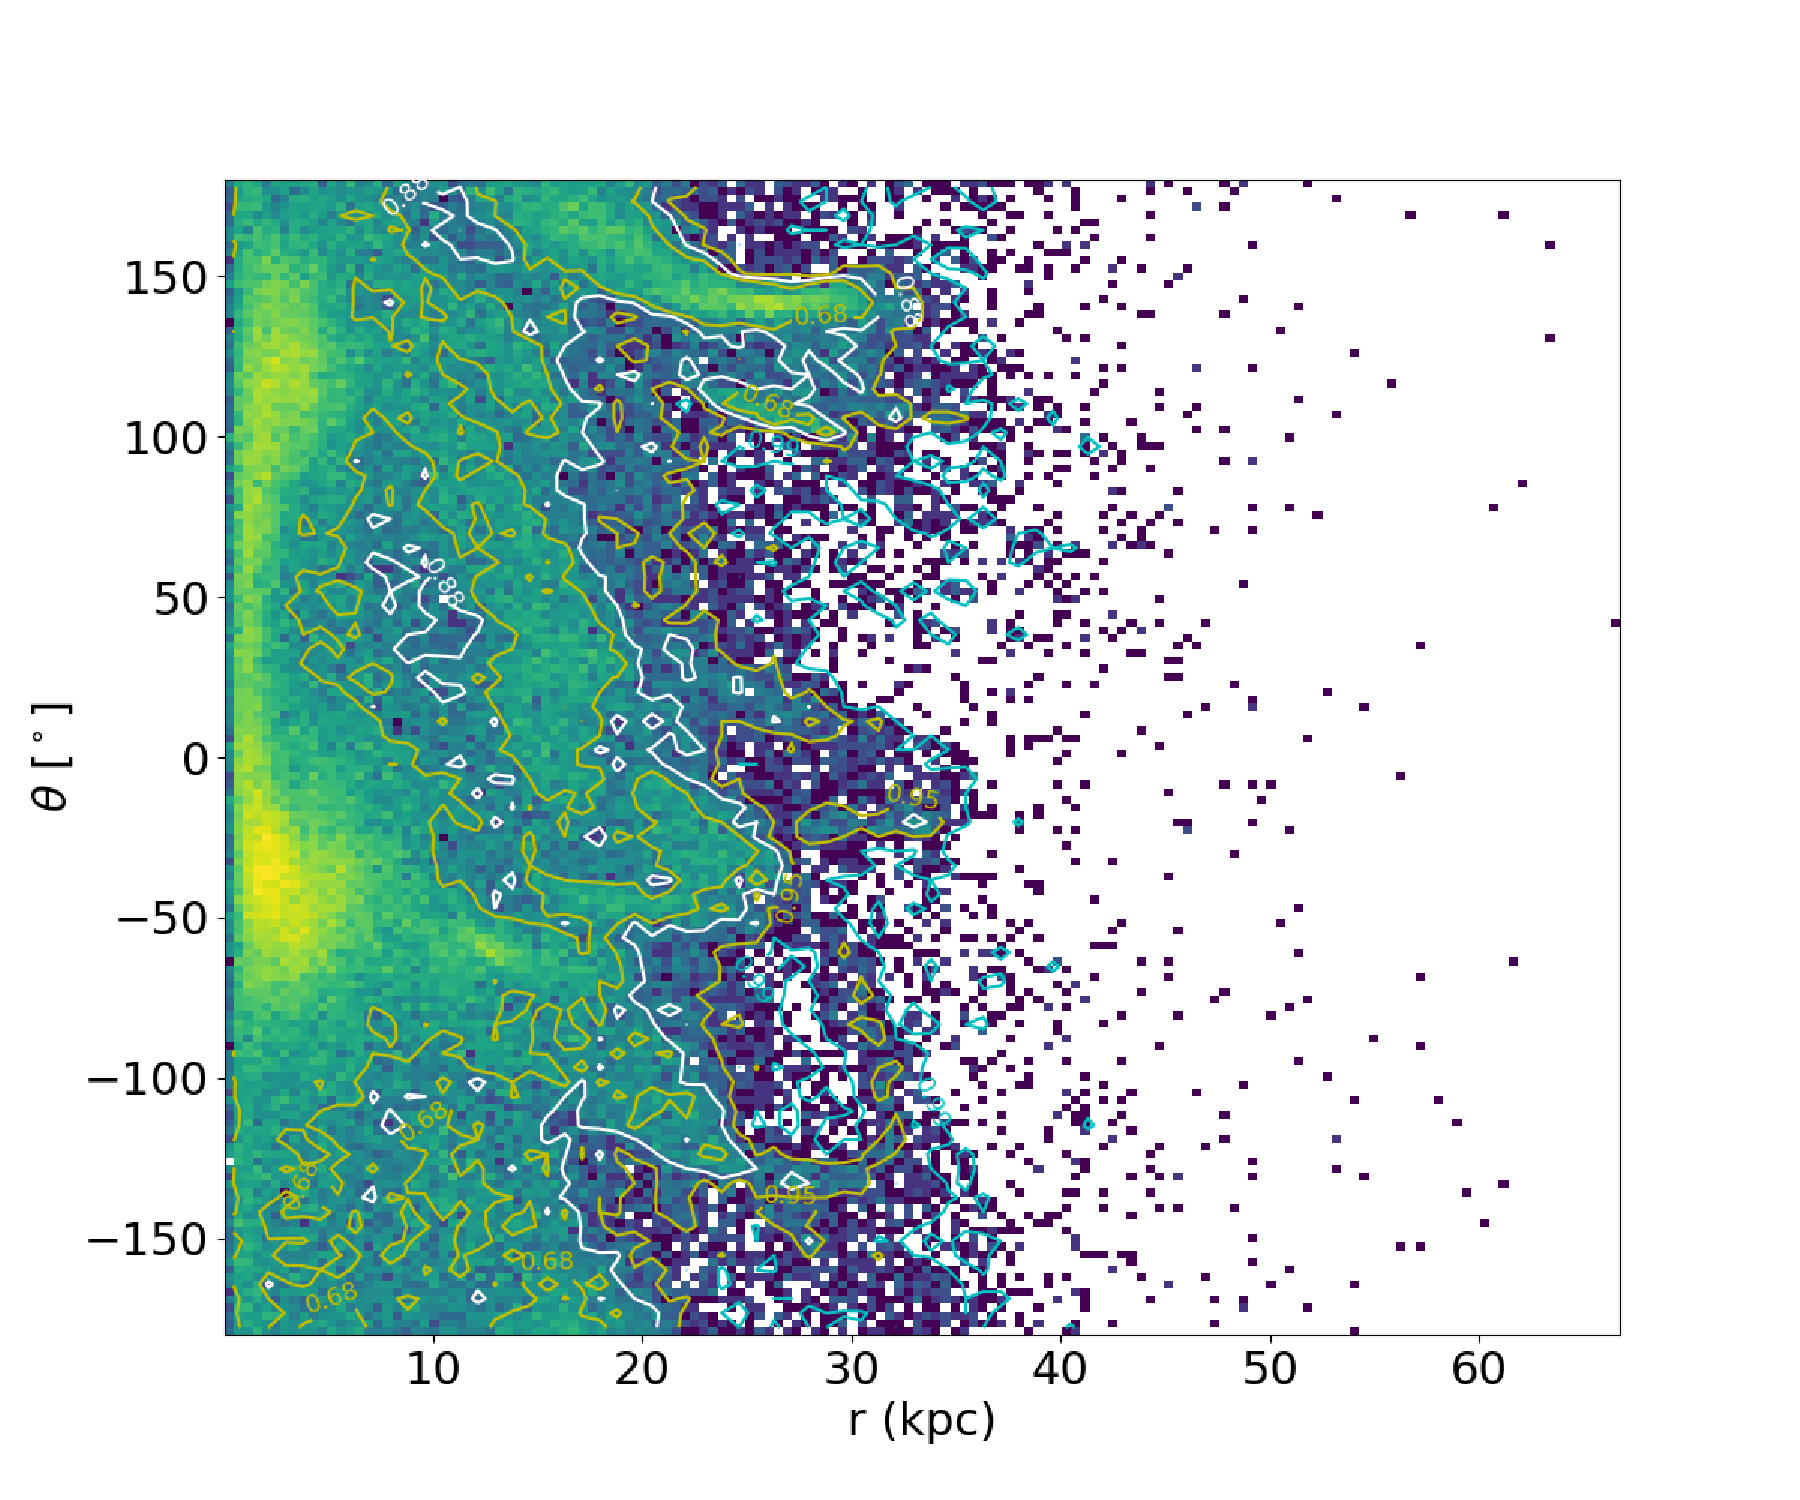
\includegraphics[width=\columnwidth]{Lab7_SpiralPhase}
  \caption{A histogram of M31 in polar coordinates $(r,\theta)$ onto
    $\mathbb{R}^2$ from Lab 7 from ASTR 400B Spring 2025 taught by
    Dr. G. Besla. This graph discretizes the stellar distribution,
    enabling us to identify the radius and principal angle of the
    bar. This analysis is used to determine the bar geometry for this
    project. By examining the density of the histogram, one can see
    that the bar appears most prominently at
    $\theta \approx -45^\circ$ and $\theta \approx 135^\circ$ Credit
    to G. Besla, R. Hoffman, R. Li, E. Patel, and myself for
    developing the code used to generate this figure.}
  \label{fig:spiral}
\end{figure}

My code will follow a modified version of the calculations from
Appendix B of \citet{dehnen:23}. This first involves separating the
galaxy into major annuli with a population of stars between
$N_\text{min}$ and $N_\text{max}$ such that the maximum and minimum
radius of each annulus are related by the equation
$R_{i,\text{max}}/R_{i,\text{min}} < 10^\Delta$. I then create
overlapping annuli halfway between the $N$ major annuli to create
$2N-1$ annuli in total. I then run a Fourier analysis of each annulus
to find the bar strength $|c_n|$ where $c_n = \sum_m
Me^{-im\theta}$. Finally, the code takes the maximum amplitude and
uses this as the strength of the bar at each snapshot.


I will generate a plot showing the evolution of the bar strength in MW
and M31 to argue that the strength of the bar is virtually
extinguished as the result of the major merger. At special snapshots
depicting the initial state, final state, and states halfway between
close encounters, I generate a plot of the bar strength with respect
to distance from the galactic nucleus, as well as density contour
plots from a face-down and cylindrical perspective that portray the
bar structure of the Milky Way and M31 as well as their merger
product. These plots allow me to address my proposal.

I expect that stars initially located further from the galactic center
will exhibit higher velocities after dispersion.

\software{This work made use of the following software packages:
  \texttt{matplotlib} \citep{Hunter:2007} and \texttt{python}
  \citep{python}. Software citation information aggregated using
  \texttt{\href{https://www.tomwagg.com/software-citation-station/}{The
      Software Citation Station}}
  \citep{software-citation-station-paper,
    software-citation-station-zenodo}.}

\bibliography{./research.bib}
\end{document}

%%% Local Variables:
%%% mode: LaTeX
%%% TeX-master: t
%%% End:
